\documentclass[letterpaper]{article}
%\usepackage{../../../LaTeX/styles/aaai}
\usepackage{aaai}
\usepackage{times}
\usepackage{helvet}
\usepackage{courier}
\usepackage{latexsym} 
\usepackage{graphicx}
\usepackage{algorithm}
\usepackage{algorithmic}
\usepackage{url}
\usepackage{colortbl}
\usepackage{color}
\usepackage{subfigure}
\usepackage{amsmath}
\usepackage{amssymb}
\usepackage{enumerate}
\usepackage[belowskip=-5pt,aboveskip=5pt]{caption}

\newtheorem{df}{Definition}
\newtheorem{notation}{Notation}
\newtheorem{theorem1}{Theorem}
\newtheorem{theorem}{Theorem}
\newtheorem{lemma}{Lemma}[section]
\newtheorem{col}{Corollary}
\newcommand{\bt}{\begin{theorem}\em}
\newcommand{\et}{\end{theorem}}
\newcommand{\Qed}{$\blacksquare$}
\newcommand{\qed}{$\Box$}
\newcommand{\proof}{{\bf Proof. }}

\newcommand{\nin}{\noindent}

\setlength{\intextsep}{10pt plus 2pt minus 2pt}

\newcommand{\bea}{\begin{eqnarray}}
\newcommand{\eea}{\end{eqnarray}}

\newcommand{\bdf}{\begin{df}\em}
\newcommand{\edf}{\end{df}}

\newcommand{\ben}{\begin{enumerate}}
\newcommand{\een}{\end{enumerate}}
\newcommand{\ie}{\item}

\newcommand{\dist}{\operatorname{dist}}

\newcommand{\avg}{\operatorname{avg}}

\definecolor{grey}{rgb}{0.4,0.4,0.4}


\numberwithin{equation}{section}
\numberwithin{theorem}{section}
\numberwithin{lemma}{section}
\numberwithin{df}{section}

\title{KthBestPick - A Strategy for Multi-Player Drafting Games}

\nocopyright

\author{Author(s) Name(s) Go Here in 12 Point Bold Times Type}
%\author{Neesha Desai, Richard Gibson, and Richard Zhao \\
%Department of Computing Science, University of Alberta \\
%Edmonton, Alberta, T6G 2E8, Canada \\
%$\{$neesha$\mid$rggibson$\mid$rxzhao$\mid$bulitko$\}$@cs.ualberta.ca}


\begin{document}

\maketitle

\begin{abstract}
A \emph{drafting game} is a game played by a set of $n$ players, where items are picked in turn without replacement from a communal collection.  Players attempt to maximize an individual end-game reward determined by the selections made by each of the players.  We present a novel strategy for playing drafting games called the KthBestPick algorithm.  KthBestPick is found to exceed a number of baseline strategies in a simple drafting game.  Furthermore, we augment an existing bot for the computer game Lux Delux (a clone of the board game Risk) with the KthBestPick drafting strategy. The algorithm is shown to greatly improve performance against the strongest opponents supplied with Lux Delux.
\end{abstract}

\section{Introduction}

% Talk about search for single agent, minimax for two-player, 0-sum, MaxN for multi-player.  Examples like chess, checkers, etc.

For the past few decades, computer games have been a popular platform for artificial intelligence research.  Many successful computer programs have been developed which play at expert levels in two-player games such as Othello \cite{Othello}, 
checkers \cite{Chinook}, chess \cite{DeepBlue}, 
and Go \cite{ComputerGo}.  These games can be handled reasonably well by classic and modern artificial intelligence techniques, such as minimax search and Monte-Carlo tree search.  However, multi-player (here and throughout meaning more than 2 players) games are less understood.  In this paper, we explore strategies for playing multi-player ``drafting'' games.  Informally, a drafting game involves players taking turns selecting from a collection of items without replacement until some end game condition has been met.  At the conclusion of the game, each player receives a reward based on the final distribution of the items; the selection order is irrelevant.  The objective for each player is to maximize the individual end game reward.  Some challenges associated with drafting games include potentially large action spaces and considering how the choices of others should affect our own.

% Also include Risk in this discussion
There are a number of games which either can be modelled as a drafting game or incorporate some kind of draft within part of the game.  A simple 2-player example is Tic-Tac-Toe.  Here, we can consider the winning player receiving a positive reward, the losing player receiving a negative reward, or both players in a draw receiving zero reward. Another example is the board game Risk by Hasbro Inc., which begins by players drafting the territories on the board until every territory has an owner.  A player should attempt to select territories so that their chance of winning the overall game is maximized.
%Drafting territories in Risk presents an additional challenge as it is not clear what selections are best in order to eventually win the overall game.  As for video games, sports simulations often include a drafting aspect.  For instance, %when playing through multiple seasons of the baseball game \textit{MLB 09: The Show} from Sony, a rookie draft takes place in between each season, where the human player and the computer opponents take turns choosing from a pool of new players who may then be added to the respective team's roster.  Another example is 
%in the new hockey game \textit{NHL 10} by EA Sports, a ``fantasy draft'' can be activated at the beginning of a season.  In a fantasy draft, all players are removed from their current teams, then selected one-by-one by the teams in the league.  Like with Risk, it can be hard to judge which selections will improve a team's chance of winning the most.  %Finally, the video game \textit{Star Wars: Empire at War} contains a drafting-type game where one can choose their ground force composition, execute ``auto-combat,'' and see the outcome of the battle.

The rest of the paper is organized as follows.  First, we formally describe drafting games and discuss related work.  We then introduce our main contribution in this paper, the KthBestPick algorithm, which is specifically designed for playing drafting games.  Next, we test out the algorithm in a simple drafting game before applying it to the opening phase of Risk.  Finally, we discuss the results and conclude with some future works.

\section{Problem Formulation}
\label{sec:Prob}

A \emph{drafting game} is a finite, deterministic, full-information sequential game played by a set of $n \geq 2$ players, which we label 1 through $n$.  The game has a finite set of actions or \emph{picks} $A$ initially available to every player, and players take turns in a predetermined order.  Once a player makes a pick, that pick is then forbidden to all players for the rest of the game.  Play continues until some predefined end game condition is satisfied or all picks in $A$ have been chosen.  At the game's conclusion, the picks made by each of the players induce a partition $Z = \{A_1, ..., A_{n}, \bar{A}\}$ of $A$, where $A_i$ is the unordered set of all picks made by player $i$, and $\bar{A}$ are the picks that were not chosen by any player.  Each player then receives a reward signal $r_i(Z)$ according to the resulting partition $Z$.  Player $i$'s objective is to make picks in such a way as to maximize $r_i(Z)$.  A drafting game does not necessarily have the notion of a winner; players simply attempt to maximize their own individual reward.  This means that depending on how the rewards are defined, a drafting game can be co-operative or competitive in nature.  On his or her turn, a player in a drafting game is faced with the following problem: Given the picks made by the players thus far, which of the remaining items should be chosen next? %Note that although at the end of the game the player with the highest reward signal is declared the winner, players may be following their own individual and independent objectives.

%\subsection{Engineering the reward signal}
%
%Some drafting games, like Tic-Tac-Toe, are stand-alone games which naturally inherit a reward signal from the rules and objectives of the game; for example, the reward signal
%\[ r_i(Z) = \left\{ \begin{array}{cl} 1 & \text{if player $i$ has 3 cells in a row in $Z$,} \\ -1 & \text{if player $j \neq i$ has 3 cells in a row in $Z$,} \\ 0 & \text{otherwise} \end{array} \right. \]
%acts as a clear objective for player $i$ to maximize in Tic-Tac-Toe.  However, in many applications, a drafting game is a precursor to a larger competition involving the same set of players.  For example, in Risk, once players draft territories, the game continues until a single player wins by occupying all territories on the map.  If we want to consider the opening draft as its own separate sub-game, it is not immediately clear what the reward signals should be.  For such a sub-game, the task is to create a reward signal $r_i(Z)$ for each player in the drafting game that correlates with the objectives of each player in the encompassing game.  Throughout this paper, we refer to these %drafting 
%games as ``drafting sub-games.''

\section{Related Work}

A widely known approach to game playing is the minimax adversarial search algorithm.  It is designed for zero-sum games involving two players, denoted Max and Min.  The Max player (assumed to be the active player) performs a search of a game tree rooted at the current state of the game.  Each leaf node of the tree is evaluated by a heuristic function, which returns a value estimating the merit of the state to Max.  These values are then backed up the tree; at nodes belonging to Max, the maximum value of the children is propagated up, whereas at nodes belonging to Min, the minimum value of the children is used.  The Max player then chooses the action leading to the child with the maximum propagated value.

\begin{table}[t]
	\centering
		\caption{The point values for an example drafting game.}
		\label{tab:KthEx}
		\begin{footnotesize}
		\begin{tabular}{|c|c|c|c|c|}
			\hline
			\bf Player $\backslash$ Action & \bfseries {\em A} & \bfseries {\em B} & \bfseries {\em C} & \bfseries {\em D} \\
			\hline
			\bf 1 & 3 & 4 & 2 & 1 \\
			\hline
			\bf 2 & 4 & 1 & 2 & 3 \\
			\hline
			\bf 3 & 4 & 2 & 3 & 1 \\
			\hline
		\end{tabular}
		\end{footnotesize}
\end{table}
% MaxN, Paranoid
% MP-Mix which extends MaxN (was used only for branching factor of 3, and for single winner games)

While minimax search is traditionally employed in many two-player games, it is not applicable to games with $n > 2$ players.  A generalization of traditional minimax search to more players is the MaxN algorithm \cite{MaxN}.  At the leaf nodes of the game tree, a heuristic function now estimates a vector of $n$ merits $(v_1, ..., v_n)$, one for each player.  At nodes belonging to player $i$, the vector with the highest merit $v_i$ is propagated up to the parent.  Thus, players are assumed to be maximizing their own individual payoffs throughout the remainder of the game.  An alternative to MaxN is the Paranoid algorithm \cite{Paranoid}, where the active player assumes that the other players are out to minimize his or her payoff with complete disregard to their own benefits.  The Paranoid algorithm is essentially equivalent to the minimax algorithm, where the other players are represented as one meta-player (Min) attempting to minimize the individual heuristic value of the active player (Max).  Finally, the MaxN and Paranoid propagation strategies can be dynamically selected according to the game situation.  This is done in the MP-Mix algorithm \cite{ZuckFelnerKraus2009}, along with a third strategy called Offensive.  However, MP-Mix was designed for games with only a single winner, which does not directly fit into our general framework of a drafting game.  On the whole, these algorithms perform best when the branching factor (i.e.~action space) is small and when there exists a good evaluation function for approximating the merits of non-terminal states.  In general, drafting games can have a very large branching factor and evaluation functions may difficult to derive; in particular, we know of no such evaluation function for the drafting stage of Risk.

An algorithm more suited for large actions spaces and requiring no evaluation function is UCT \cite{UCT}, a Monte Carlo planning algorithm that has commonly been used in general game playing, for example in CadiaPlayer \cite{Cadia}.  UCT tries to intelligently bias the game tree by simulating games that focus on appealing branches of the tree.  At each step, UCT builds upon the sparse game tree from the previous simulations by selecting an action $a$ at state $s$ to expand by
\[ a = \text{argmax}_{a'} \left( Q(s,a') + c \sqrt{ \log n(s) / n(s,a') } \right), \]
where $Q(s,a)$ is the estimated value of taking $a$ at $s$, $c$ is an exploration constant, $n(s)$ is the number of times $s$ has been visited, and $n(s,a)$ is the number of times $a$ has been taken in $s$.  For drafting games, we view $Q(s,a)$ as the average of the reward signal $r_i(Z)$ (assuming it is player $i$'s turn at $s$) seen on all simulations through $s$ where action $a$ was taken.  On each simulation, UCT adds one new node to the game tree and then randomly plays out the rest of the game.  % from that node to obtain $r(Z)$, which is then propagated up the tree.  %If UCT was allowed to perform an infinite number of roll outs and the exploration constant was constant,  UCT would become strictly Monte Carlo planning.  We refer to UCT as UCT$(x,c)$, where $x$ is the number of simulations run and $c$ is the exploration constant. 
After running numerous simulations from the current state $s$, UCT takes the action $\text{argmax}_{a}Q(s,a)$.

Finally, there has been some progress on the problem of drafting in sports leagues.  Many professional sports use a drafting procedure where teams sequentially select entry-level players based on the teams' current needs and scouting reports of the players' skills.  Brams and Straffin \cite{PrisonAndDrafting} examine very small games where each team has its own order of preference of the entering players.  They use a MaxN-type approach to find optimal drafting strategies, but hint that the approach is ill-advised for larger drafts due to a prohibitively large branching factor.  In addition, Fry et.~al \cite{SportsDrafting} solve a deterministic dynamic programming problem through linear programming to determine a team's best drafting strategy and apply it to a fantasy football draft.  However, a key ingredient in their model is that each team has positional (quarterback, running back, etc.) needs and limits its picks to a fixed number of players for each position.  In general, we are not concerned with items being categorized or restricted to competitors in any way.

\section{The KthBestPick Algorithm}
\label{sec:drafting}

\begin{algorithm}[t]
	\caption{KthBestPick($node$, $N$, $h$, $m_0$, ..., $m_{n-1}$)}
	\label{alg:kth}
	\begin{footnotesize}
	\begin{algorithmic}[1]
		\STATE $rankedPicks \gets $ sort($node$.getActions(), $h$)
		\STATE $p \gets node$.getActivePlayer()
		\FOR{$k$ from min($node$.getNumPicksLeft(p)$-1$, $N$) to $0$}
			\STATE $pick \gets rankedPicks(k)$
			\STATE $betterPicks \gets rankedPicks(0..k-1)$
			\STATE $child \gets node.$getChild($pick$)
			\STATE $makeThisPick \gets $ TRUE
			\WHILE{$betterPicks$ is not empty}
				\IF{$child$.isGameOver()}
					\STATE $makeThisPick \gets $ FALSE
					\STATE BREAK
				\ENDIF
				\STATE $p \gets child$.getActivePlayer()
				\STATE $nextPick \gets m_p(child)$
				\STATE $child \gets child.$getChild($nextPick$)
				\IF{$nextPick \in betterPicks$}
					\IF{$p = node$.getActivePlayer()}
						\STATE $betterPicks.$remove($nextPick$)
					\ELSE
						\STATE $makeThisPick \gets $ FALSE
						\STATE BREAK
					\ENDIF
				\ENDIF
			\ENDWHILE
			\IF{$makeThisPick$}
				\RETURN{$pick$}
			\ENDIF
		\ENDFOR
	\end{algorithmic}
	\end{footnotesize}
\end{algorithm}

% Describe UCT, specifically for multi-player games (like drafting games)

% May want to discuss theoretical properties of UCT (converges to Nash equilibrium?)

% Perhaps mention UCT being used in GGP (plus reference)?

%Monte-Carlo tree search algorithms, such as UCT \cite{UCT}, are a different approach to game playing than minimax-type methods.  Simply put, thousands of games are simulated to completion, and each node's value is set to the average of the outcomes which passed through that node.  As game tree sizes typically grow exponentially in their branching factor, minimax-type algorithms must often rely on an accurate heuristic function at non-terminal nodes due to memory or time constraints.  Monte-Carlo tree search, on the other hand, needs no heuristic function and receives an unbiased estimate of the value of each action.  Because of this, UCT is often preferred in games with large action spaces or which lack a quality heuristic function, and has had much success in Computer Go \cite{ComputerGo}.  As drafting games typically have large, initial action spaces and lack a general heurstic function, we have implemented UCT as a drafting strategy.  UCT is also used as a base for our new algorithm, KthBestPick (see Section \ref{sec:KthBestPick}).

%\begin{figure}[t]
%	\centering
%	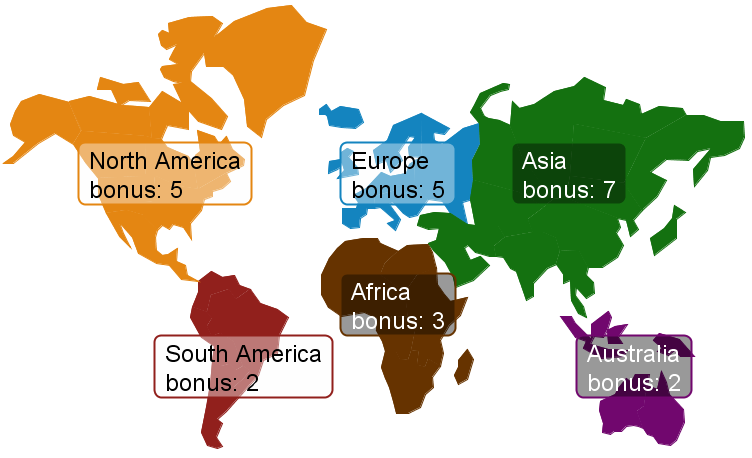
\includegraphics[scale=0.325]{figs/Conts.png}
%	\caption{The layout of the Risk board and the continent reinforcement bonuses, modified from Lux Delux.}
%	\label{fig:Conts}
%\end{figure}

%\subsection{The KthBestPick Algorithm}
%\label{sec:KthBestPick}
% kthBestPick search

Before introducing the algorithm, we consider a small example to build up some intuition for KthBestPick.  Consider the drafting game with four actions, $A$, $B$, $C$, and $D$, and three players, 1, 2, and 3.  Players pick in numerical order until all actions have been picked (thus player 1 gets two picks).  For each action and each player, we associate a point value that that player receives for making that pick.  A player's reward at the end of the game is simply the sum of the points of his or her picks.  Suppose the point values are as given in Table \ref{tab:KthEx}, and let's assume that we are player 1.  If we rank picks according to the point values for us only, then $B$ would appear to be the best pick (4 points) and $A$ the second best (3 points).  Following this heuristic alone would have us pick $B$.  Now if players 2 and 3 are playing optimally, player 2 will follow by picking $A$, then player 3 will pick $C$.  This forces us to pick $D$, leaving us with a reward of $4 + 1 = 5$.  However, assuming our opponents play optimally, we can see that picking $A$ first will lead player 2 to pick $D$ and player 3 to pick $C$, leaving us to pick $B$ with our last pick.  In this case, we end the game with a reward of $3 + 4 = 7$, a better result.  KthBestPick is designed to act intelligently in situations like this.

At each turn, KthBestPick uses a heuristic function to rank the available picks from best (rank 0) to worst.  Then, it estimates the most inferior pick of rank $k$ that we may choose so that we eventually pick all $k$ better-ranked actions with our later picks.  This is done using opponent models to predict the play of the other players. %, which may or may not be different from the heuristic function.

\begin{figure}[t]
	\centering
	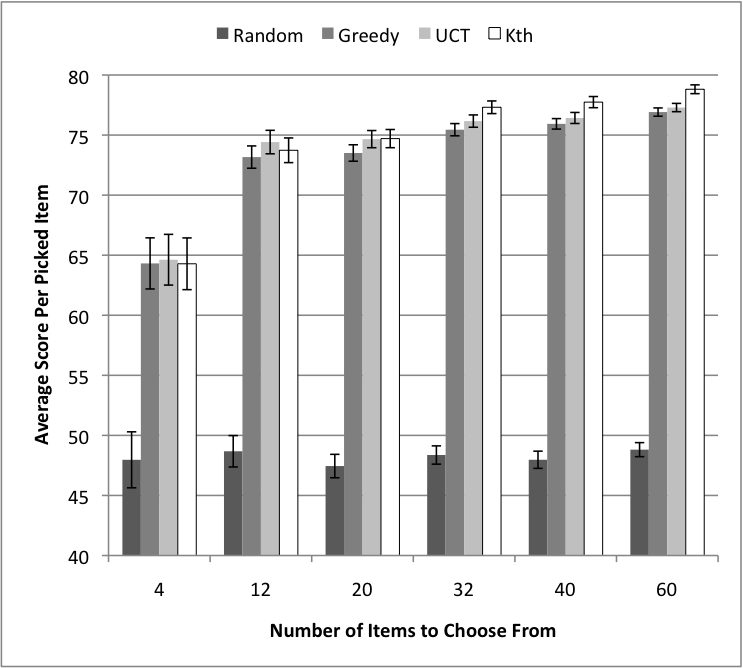
\includegraphics[scale=0.55]{figs/TableDraft.png}
	\caption{The average value per pick achieved in the simple drafting game by each of the four strategies.  Error bars indicate 95\% confidence intervals.}
	\label{fig:SimpleDraftGraph}
\end{figure}

Algorithm \ref{alg:kth} gives the pseudocode for KthBestPick, which takes in the current state $node$, a number of top-ranked picks to consider $N$, a heuristic function $h$, and a sequence of opponent models $m_0, ..., m_{n-1}$ (one for each player) as parameters.  We first rank the actions according to the heuristic function (line 1).  Next, $k$ is set to $N$ or one fewer than the number of picks remaining for the active player (line 3) (as we do not have enough picks to consider more inferior actions), whichever is smaller.  Then, we set our potential pick to the action ranked $k$ (line 4), construct a list containing all of the superior picks (line 5), and initialize $child$ to point to the child node associated with this potential pick.  To determine if this pick is desired, we repeatedly find each of the next picks made by the players according to the opponent models (line 14).  Each model returns the action believed to be picked by the active player at the passed in node.  After updating our $child$ pointer to follow this next pick (line 15), we check if the pick is in our list of superior actions (line 16).  If it is, there are two possible cases.  If the pick was made by the caller of the algorithm (line 17), then this is allowed; we remove the pick from the superior list (line 18) and continue.  However, if the pick was made by another player, then we abandon our potential pick (lines 20 and 21), decrement $k$ (line 3), and now consider the new potential pick ranked $k$ (line 4 again).  If the list of superior picks ever becomes empty (line 8), this indicates that the original active player is predicted to pick all of the superior actions, and so we return the current potential pick (line 26).  However, if the game ends while superior actions remain unclaimed (line 9), we instead abandon the potential pick (lines 10 and 11). 

% Possible heuristic functions: learn one based on a number of features describing the current state-action space, or can use MaxN-MC.
There are a number of different possibilities for the heuristic function and the choice is usually dependent on the particular drafting game.  For instance, in the example game in Table \ref{tab:KthEx}, ranking items according to the value to us is a straightforward heuristic.  If the game does not lend itself to such a heuristic, another choice is to use UCT.  UCT stores a value $Q(node,pick)$ for each available action estimating the merit of selecting $pick$, allowing the actions to be sorted as necessary.

% Possible opponent models: KthBestPick (in practice, keep track of repeated calls in one state, and truncate the game to a fixed maximum number of picks remaining), if repeated games then could try to learn an opponent model.  Typically will not be given the explicit opponent drafting strategies.
As for the opponent models, again there are a few options.  Firstly, we should use KthBestPick as the opponent model for our own play, since we know this is the strategy being used to make our picks.  Typically for the other players, however, we will not be given their explicit drafting strategies.  The simplest approach would be to assume that the opponents are also using KthBestPick to make decisions with an appropriate self-centered heuristic function.  This turns line 14 of Algorithm \ref{alg:kth} into a recursive call, and in this case, KthBestPick can be very costly in computation time.  We can combat this by iteratively increasing $N$ until returning a pick is necessary.  Finally, if we are fortunate enough to have obtained the strategies of our opponents, we can simply pass these into the algorithm.

Note that in the example game described in Table \ref{tab:KthEx}, UCT will also conclude that picking $A$ first is a better move, but only after a number of simulations.  KthBestPick, on the other hand, finds the solution with just one ``simulation.''

%\section{Theoretical Analysis}
%
%\begin{theorem1}
%	\label{thm:Kth}
%	KthBestPick always returns an action.
%\end{theorem1}
%\begin{proof}
%Firstly, the while loop in Algorithm \ref{alg:kth} (line 8) is not infinite.  This is because drafting games are finite and acyclic (no state can be repeated), and each pass through the loop makes one more action.  Thus the condition at line 9 must eventually be met.  Now consider the value of $k$ in the for loop at line 3.  If $k = 0$, then the $betterPicks$ list is set to empty (line 5), implying that the while loop condition (line 8) is false and we return our pick (line 26).
%\end{proof}

\begin{table}[t]
	\centering
		\caption{The weights for features (ii), (iii), and (iv) as computed in Weka.} 
		\label{tab:MoreScoring}
		\begin{footnotesize}
		\begin{tabular}{|c|c|}
			\hline
			\textbf{Feature} & \textbf{Points} \\
			\hline
			First to play & 13.38 \\
			\hline
			Second to play & 5.35 \\
			\hline
			Each unique enemy neighbour & -0.07 \\
			\hline
			Each ordered pair of friendly neighbours & 0.48 \\
			\hline
		\end{tabular}
		\end{footnotesize}
	
\end{table}

\section{Empirical Evaluation}

In this section, we first apply KthBestPick to a simple drafting game and compare it to some other strategies.  We then use the algorithm to select territories in the opening phase of Risk to improve overall play.

\begin{figure*}[t]
	\centering
	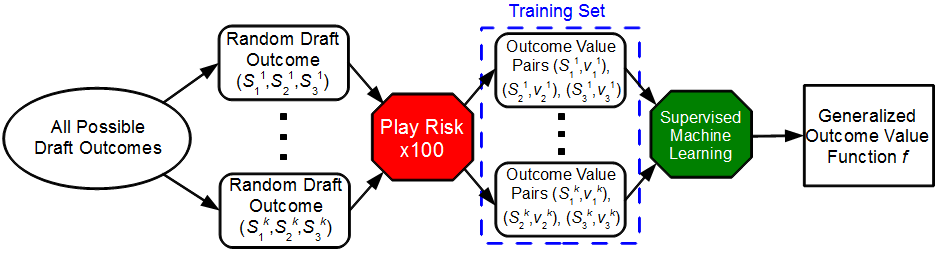
\includegraphics[scale=0.5]{figs/MachineLearner.png}
	\caption{The process described for obtaining a general function $f$ for estimating the merit of each feature set (adapted from \cite[Figure 5.1]{GregLeeThesis}).}
	\label{fig:MachLearn}
\end{figure*}

\subsection{A Simple Drafting Game}

We generated several 4-player drafting games similar to the example game given in Table \ref{tab:KthEx}.  The game starts with $k$ available actions to the 4 players, labeled 1 through 4, who follow the turn ordering $(1,2,3,4,1,2,3,4,...)$.  For each action and each player, we assign a uniformly random integer value between 0 (inclusive) and 100 (exclusive) that that player receives for taking that action, meaning that the items are valued differently among the players.  The game ends once all actions have been selected and each player's end game reward is the sum of the values of his or her picks.   

The KthBestPick strategy was pitted against a greedy strategy that simply chooses the remaining action with the highest point value for itself, UCT with exploration constant $c = 250$ (determined to be a good choice through preliminary experiments), and a random strategy.  KthBestPick simply uses the straightforward personal integer value as its heuristic to rank the picks.  For example, the ordering of the items in Table \ref{tab:KthEx} (assuming KthBestPick is player 1) would be $(B,A,C,D)$.  In addition, we assume KthBestPick does not know the strategies of the other players, resorting to the assumption that all opponents also use KthBestPick to make selections.  To fairly compare KthBestPick and UCT, we enforced a time limit per turn of $133 \left \lceil \ell / 4 \right \rceil$ milliseconds, where $\ell$ is the number of actions remaining to be picked.  KthBestPick is iteratively called, starting with $N = 1$ and increasing by one each iteration, and returns the pick from the latest finished call once time expires.  UCT just runs simulations until time expires before returning its desired action.

We used six different sizes of games between $k=4$ and $k=60$ as shown along the x-axis in Figure \ref{fig:SimpleDraftGraph}.  For each size, we generated 25 random assignments of the $4k$ integer values.  Each of these 25 drafting games were then played $24$ times, once for each of the $4!$ orderings of the players.  Figure \ref{fig:SimpleDraftGraph} shows, for each $k$, the average value earned per pick across all $25 \cdot 24 = 600$ games played.  COMPUTER SPECS?  For the smaller games with $k=4,12,$ and $20$, we see that Greedy, UCT, and KthBestPick all earn roughly the same amount of value per pick as the confidence intervals overlap.  For $k=4$, each player only gets to pick one action, and thus the Greedy strategy is clearly optimal.  For $k=12$ and $20$, Greedy still performs well enough for these generated games, perhaps because the random player cannot disrupt Greedy's ``plan.''  For smaller $k$, UCT can simulate many games to completion and calculate a good estimate of which pick is best in the long term.  However, for larger $k$, each UCT simulation takes more time to complete and has more branches of the game tree to explore, leading to a less accurate assessment.  The Greedy strategy also becomes less viable as situations like those in Table \ref{tab:KthEx} can occur more frequently.  On the other hand, KthBestPick is much less affected by a larger $k$ as it only traverses the top of the game tree, and can see past the mistakes prone to Greedy.  Despite the presence of an unpredictable random opponent, KthBestPick is the preferred strategy in our games with $k=32,40,$ and $60$.

\subsection{Risk}

Risk is a strategy board game for two to six players where the objective is to occupy all 42 territories in 6 continents on the board.  %The territories are divided into 6 continents
%, with 4 territories in both Australia and South America, 6 in Africa, 7 in Europe, 9 in North America, and 12 in Asia.  Figure \ref{fig:Conts} depicts their arrangement on the board.  In the standard rules, players first take turns selecting the territories until all have been chosen (the drafting sub-game).  After each player places their initial armies among their selected territories, players then take turns until only one player remains.  On a turn, in sequence a player may place reinforcements, conduct attacks on opposing territories, and tactically maneuver armies amongst owned territories.  Attacks are resolved by dice rolls, where the number of dice is dependent on the number of attacking and defending armies.  A player reduced to zero armies on the board is eliminated from the game.  Players receive one reinforcement army for every three territories owned and receive bonus reinforcements for owning entire continents (as depicted in Figure~\ref{fig:Conts}) or trading in cards earned by conquering territories. Full rules can be found on-line\footnote{\url{http://www.hasbro.com/common/instruct/Risk.pdf}}.
%as labelled in Figure \ref{fig:Conts}.  
In the standard rules, players first take turns selecting the territories until all have been chosen.  After players place their initial armies among their selected territories, players then take turns placing reinforcements, conducting attacks, and tactically maneuvering armies until only one player remains.  %On a turn, in sequence a player may place reinforcements, conduct attacks on opposing territories, and tactically maneuver armies amongst owned territories.  Attacks are resolved by dice rolls, where the number of dice is dependent on the number of attacking and defending armies.  
%A player reduced to zero armies on the board is eliminated from the game.  
%Players receive one reinforcement army for every three territories owned, and receive bonus reinforcements for owning entire continents (as depicted in Figure~\ref{fig:Conts}) or trading in cards earned by conquering territories. 
Full rules can be found on-line \cite{Risk}. %\footnote{http://www.hasbro.com/common/instruct/Risk.pdf}.

The Lux Delux \cite{Lux} %\footnote{http://sillysoft.net/lux/} 
game provides a computer version of Risk, along with several AI programs (bots) with source code to play against, all of which are rule-based.  Each of the included bots has an associated difficulty and a general playing style.  For example, ``Quo'' is a difficult bot that tries to form a cluster of adjacent territories and methodically expand that cluster.  We use the Lux Delux environment in all of our computations and experiments.

In this paper, we are only concerned with how to play the opening draft of Risk.  While strategies for the other phases of Risk are interesting and have been researched (\cite{RiskBots}, \cite{ZuckFelnerKraus2009}), we do not investigate these here.  Instead, we simply use the Quo bot's rules for our own post-draft play.  In addition, we decide to focus only on 3-player Risk, as this moves beyond a 2-player zero-sum game and incorporates the multi-player aspect of drafting games.  It is also arguably more strategically demanding compared to playing with more players because each player must make more selections per draft.

\begin{table*}[t]
 \centering
      \caption{The weights for features of type (i), as computed in Weka.  Rows denote continents and columns denote territory counts.  Weights denoted with a * are derived through linear extrapolation.}
    \label{tab:ContScoring}
    \begin{footnotesize}
    \begin{tabular}{|c|c|c|c|c|c|c|c|c|c|c|c|c|c|}
    	\hline
    	  & \bf 0 & \bf 1 & \bf 2  & \bf 3 & \bf 4 & \bf 5 & \bf 6 & \bf 7 & \bf 8 & \bf 9 & \bf 10 & \bf 11 & \bf 12 \\
    	 \hline
    	\bf Australia & 2.97 & 0 & 8.45 & 9.99 & 10.71 & - & - & - & - & - & - & - & - \\
    	\hline
    	\bf South Amer. & 0.69 & 1.23 & 3.90 & 0 & 17.72 & - & - & - & - & - & - & - & - \\
    	\hline
    	\bf Africa & 14.40 & 12.87 & 10.72 & 7.16 & 1.23 & 0 & 29.80 & - & - & - & - & - & - \\
    	\hline
    	\bf North Amer. & 3.11 & 0.98 & 0 & 2.17 & 7.15 & 19.35 & 24.82 & 24.10 & 36.15 & 48.20* & - & - & - \\
    	\hline
    	\bf Europe & 42.44 & 45.11 & 43.11 & 43.77 & 41.35 & 50.77 & 43.85 & 36.93* & - & - & - & - & - \\
    	\hline
    	\bf Asia & 27.10 & 23.90 & 23.61 & 23.10 & 23.61 & 23.68 & 19.32 & 15.63 & 17.43 & 13.84 & 10.25* & 6.66* & 3.07* \\
    	\hline
    \end{tabular}
    \end{footnotesize}
\end{table*}

We would like to use KthBestPick to select territories during the opening phase of Risk.  Since we do not know of a simple ranking of Risk territories, we decide to use UCT as the heuristic $h$ for ranking picks.  This, in a way, makes KthBestPick a ``meta-strategy'' on top of UCT.  The game of Risk, however, does not appear to be well-suited to numerous random simulations since games are typically very long.  Instead of simulating entire games, we will instead simulate only the initial drafting portion of the game.  We do this by evaluating each draft outcome with a numerical score that we hope estimates our probability of winning the entire game of Risk from that draft outcome.  In terms of our drafting game framework, this numerical score corresponds to the reward signal $r_i(Z)$ of the draft outcome $Z$ which we play to maximize in the draft.  Finally, we calculate this reward function $r_i(Z)$ using supervised machine learning, which we now describe.

Our learning technique is closely related to that introduced by Lee.  In his thesis \cite{GregLeeThesis}, Lee combines single-agent heuristic search with a machine-learned fitness function to pick a set of actions from a large library, which an agent is then restricted to in a Markov Decision Process.  The objective is to find a small set of actions which enable the agent to behave as close to optimal as possible in its domain, relative to having access to the entire library of actions.  Our approach here can be seen as an extension of Lee's work from a single-agent problem to a competitive multi-agent problem, where we replace single-agent search with an adversarial method. 

%\section{A Machine-Learned Reward Signal}

%Our objectives in this paper include both determining what strategies are desirable in drafting games, and finding a strategy in the Risk drafting sub-game that can improve our chances of winning in the full game of Risk.  The latter problem suffers from a few complications.  First, the merit of a strategy may highly depend on how we act in the rest of the Risk game.  For instance, a drafting strategy that primarily selects territories in North America would not be advisable to play with a post-draft strategy that plays to own Australia at all costs.  %With this post-draft strategy, it would make more sense to simply select territories in Australia rather than North America during the draft.  
%Secondly, as mentioned previously, it is not easy to classify a draft outcome $Z$ as either ``good'' or ``bad'' for player $i$.  This makes it difficult to guide drafting selections towards desirable outcomes.  What we are lacking is a reward signal $r_i(Z)$ that approximates player $i$'s chances of winning from $Z$ when following a given post-draft strategy.  In this section, we describe how we used supervised machine learning to create such a reward signal.

% Meta-models for reducing action space



%\begin{figure}[t]
%	\centering
%	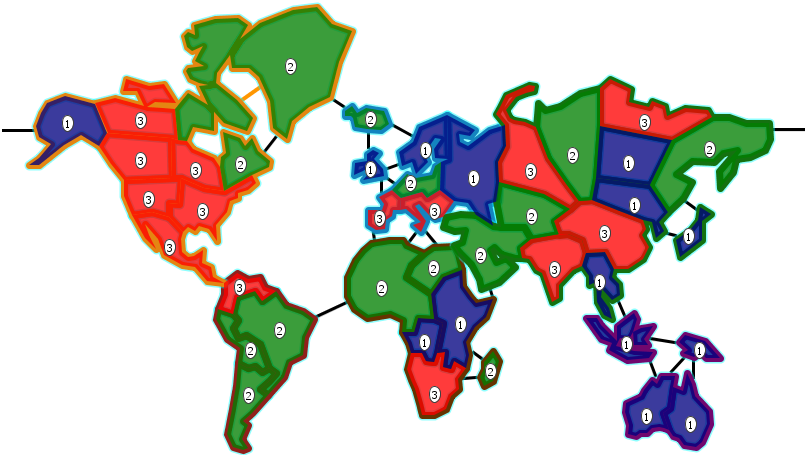
\includegraphics[scale=0.3]{figs/DraftExample.png}
%	\caption{An example of a draft outcome.  The territories picked by players 1, 2, and 3 are blue, green, and red respectively.  Territories connected by a line are also considered adjacent or bordering. Modified from Lux Delux.}
%	\label{fig:DraftExample}
%\end{figure}

We manually identified a number of features that are tactically important in draft outcomes of Risk.  Many of these features are inspired by the calculation of highest ``bids'' \cite{RiskBots}.  For each player, our features are described by: (i) for each continent, the number of territories owned in that continent; (ii) when the player plays in the turn order; (iii) the number of distinct territories owned by other players which border owned territories (enemy neighbours); and (iv) the number of distinct ordered pairs of owned territories which are adjacent (friendly neighbours).  Our process for estimating the merit of a feature set is depicted in Figure \ref{fig:MachLearn}.  First, we collect many draft outcomes, each obtained by randomly assigning all 42 territories evenly among the three players.  Then, for each draft outcome, 100 games are played to completion where each player follows the post-draft strategy of the Quo bot.  Each player $i$, $i=1,2,3$, has a set of features $S_i$ associated with each outcome.  Each feature set is assigned a value $v_i \in \{0,1,...,100\}$ equal to the number of games that player $i$ eventually won from the associated draft outcome.  This provides a collection of feature set value pairs $\{(S_i, v_i)\}$ of size equal to three times the number of draft outcomes collected.  Next, supervised machine learning is applied to obtain a general function
\[ f: S \mapsto v \in \textbf{R} \] 
that estimates the merit of the feature set $S$ when following Quo's post-draft strategy.  Finally, for a draft outcome $Z = (A_1,A_2,A_3,\emptyset)$ with $A_i$ being the set of player $i$'s picks, we calculate $v_i = f(S_i)$ where $S_i$ is the feature set associated with $A_i$, and define the reward signal for player $i$ to be
\[ r_i(Z) = v_i^+ / \left(v_1^+ + v_2^+ + v_3^+\right), \]
where $v_i^+ = \max(0, v_i)$.  %Note that even though all training values $v_i$ are nonnegative, a learner could allow $f$ to be negative and so we take the max to keep the sign of $r_i(Z)$ correct.  
Thus, $r_i(Z) \in [0, 1]$ approximately measures the value of our selections relative to the picks made by the other players.  The hope is that $r_i(Z)$ is a good estimate of player $i$'s chance of winning from $Z$.
%Thus, to maximize reward, the objective of each player is to maximize the estimated merit of her selections while minimizing those of her opponents.

Our general function $f$ is computed off-line from $7364$ random draft outcomes for a total of $22092$ $(S,v)$ pairs.  We use Weka \cite{Weka} to weight each individual feature using Weka's linear regression classifier (with no attribute selection), where features (i) and (ii) are represented as nominal features and features (iii) and (iv) are  numeric.  These weights are displayed in Tables \ref{tab:ContScoring} and \ref{tab:MoreScoring}.  However, there are some features which do not appear in any of the $22092$ feature sets because of their unlikeliness of occurring through random drafting; for instance, there were no cases where one player owned all 9 territories of North America.  The weights of these features are calculated through linear extrapolation of the closest two continent counts for the associated continent.  %For instance, the weight for owning all 9 territories in North America is calculated from the weights for owning 8 territories and 7 territories in North America via
%\[ 36.1487 + (36.1487 - 24.0969) = 48.2005. \]  
%Note that only in rare cases will $f$ be negative (lots of enemy neighbours and low scores elsewhere).  
%SHOW DIAGRAM OF LINEAR EXTRAPOLATION FOR NORTH AMERICA?  ONLY IF THERE'S ROOM.

%\begin{table*}[t]
%  \begin{center} 
%   \caption{The weights for features of type (i), as computed in Weka.  A * denotes weights derived through linear extrapolation.}
%    \label{tab:ContScoring}
%    \begin{tabular}{|c|c|c|c|c|c|c|}
%    	\hline
%    	\bf Number of Territories & \bf Australia & \bf South America & \bf Africa & \bf North America & \bf Europe & \bf Asia \\
%    	\hline
%    	\bf 0 & 2.972 & 0.6904 & 14.3958 & 3.1092 & 42.4404 & 27.0974 \\
%    	\hline
%    	\bf 1 & 0 & 1.232 & 12.8728 & 0.9766 & 45.1071 & 23.9027 \\
%    	\hline
%    	\bf 2 & 8.4532 & 3.8997 & 10.7207 & 0 & 43.1116 & 23.6086 \\
%    	\hline
%    	\bf 3 & 9.9902 & 0 & 7.1637 & 2.1682 & 43.7726 & 23.1026 \\
%    	\hline
%    	\bf 4 & 10.7097 & 17.7184 & 1.23 & 7.1541 & 41.3515 & 23.6086 \\
%    	\hline
%    	\bf 5 & - & - & 0 & 19.3505 & 50.7666 & 23.6794 \\
%    	\hline
%    	\bf 6 & - & - & 29.796 & 24.8183 & 43.8472 & 19.3189 \\
%    	\hline
%    	\bf 7 & - & - & - & 24.0969 & 36.9278* & 15.6257 \\
%    	\hline
%    	\bf 8 & - & - & - & 36.1487 & - & 17.4338 \\
%    	\hline
%    	\bf 9 & - & - & - & 48.2005* & - & 13.8433 \\
%    	\hline
%    	\bf 10 & - & - & - & - & - & 10.2528* \\
%    	\hline
%    	\bf 11 & - & - & - & - & - & 6.6623* \\
%    	\hline
%    	\bf 12 & - & - & - & - & - & 3.0718* \\
%    	\hline
%    \end{tabular}
%  \end{center}
%\end{table*}

%\begin{table*}[t]
%  \begin{center} 
%   \caption{The weights for features of type (i), as computed in Weka.  A * denotes weights derived through linear extrapolation.}
%    \label{tab:ContScoring}
%    \begin{tiny}
%    \begin{tabular}{|c|c|c|c|c|c|c|c|c|c|c|c|c|c|}
%    	\hline
%    	  & \bf 0 & \bf 1 & \bf 2  & \bf 3 & \bf 4 & \bf 5 & \bf 6 & \bf 7 & \bf 8 & \bf 9 & \bf 10 & \bf 11 & \bf 12 \\
%    	 \hline
%    	\bf Australia & 2.972 & 0 & 8.4532 & 9.9902 & 10.7097 & - & - & - & - & - & - & - & - \\
%    	\hline
%    	\bf South America & 0.6904 & 1.232 & 3.8997 & 0 & 17.7184 & - & - & - & - & - & - & - & - \\
%    	\hline
%    	\bf Africa & 14.3958 & 12.8728 & 10.7207 & 7.1637 & 1.23 & 0 & 29.796 & - & - & - & - & - & - \\
%    	\hline
%    	\bf North America & 3.1092 & 0.9766 & 0 & 2.1682 & 7.1541 & 19.3505 & 24.8183 & 24.0969 & 36.1487 & 48.2005* & - & - & - \\
%    	\hline
%    	\bf Europe & 42.4404 & 45.1071 & 43.1116 & 43.7726 & 41.3515 & 50.7666 & 43.8472 & 36.9278* & - & - & - & - & - \\
%    	\hline
%    	\bf Asia & 27.0974 & 23.9027 & 23.6086 & 23.1026 & 23.6086 & 23.6794 & 19.3189 & 15.6257 & 17.4338 & 13.8433 & 10.2528* & 6.6623* & 3.0718* \\
%    	\hline
%    \end{tabular}
%    \end{tiny}
%  \end{center}
%\end{table*}

%We now show how to use Tables \ref{tab:ContScoring} and \ref{tab:MoreScoring} to compute $r_i(Z)$ for the draft outcome given in Figure \ref{fig:DraftExample}.  Player 1 (blue) has 4 territories in Australia, 0 in South America, 2 in Africa, 1 in North America, 3 in Europe, and 4 in Asia.  In addition, player 1 has 18 distinct enemy neighbours and 22 ordered pairs of friendly neighbours.  Assuming player 1 is first to play, $f(S_1)$ is computed as
%\begin{eqnarray*}
%% 	f(S_1) &=& [10.7097 + 0.6904 + 10.7207 \\ && +\ 0.9766 + 43.7726 + 23.6086] \\ &&+\ [13.3818 + 18(-0.0719) + 22(0.4799)] \\
%% 				 &=& 113.124,
% 	f(S_1) &=& [10.71 + 0.69 + 10.72 + 0.98 + 43.77 \\ &&+\ 23.61] + [13.38 + 18(-0.07) + 22(0.48)] %\\
%% 				 &=& 113.12,
%\end{eqnarray*}
%where the values in the first set of brackets are from Table \ref{tab:ContScoring} and the second set of brackets are from Table \ref{tab:MoreScoring}.  This gives $f(S_1) = 113.12$.  We can similarly compute the values of the feature sets for player 2 (green) and player 3 (red) as %$f(S_2) = 89.4739$ and $f(S_3) = 119.6547$ 
%$f(S_2) = 89.47$ and $f(S_3) = 119.65$ respectively, where player 2 is second to play.  Finally, $r_i(Z)$ is computed via $r_i(Z) = f(S_i) / \left(f(S_1) + f(S_2) + f(S_3) \right)$, giving us %$r_i(Z) = \{0.3509, 0.2776, 0.3712\}$ 
%$r(Z) = \{0.35, 0.28, 0.37\}$.

%\section{Empirical Evaluation}

%
%In this section, we describe the drafting game we call ``Fantasy Risk,'' a stand-alone drafting game that mimics the drafting sub-game of standard Risk.  We then compare our drafting approaches in Fantasy Risk.  To end the section, we combine UCT with Quo's post-draft strategy and face off against the most difficult bots provided with Lux Delux in full games of Risk.
%
%\subsection{Fantasy Risk}
%
%% Explain fantasy risk, plus give scoring table.
%In Fantasy Risk, players take turns selecting from the 42 territories on the Risk board until all territories have been claimed, just as in the beginning of standard Risk.  Then, the game immediately ends and the players receive rewards according to our machine-learned reward signal described in the previous section.  Playing Fantasy Risk allows us to better analyze our different drafting strategies without worrying about the dynamics and variance of post-draft Risk.  
%
%\subsection{Comparison of Algorithms in Fantasy Risk}
%
%% Run experiments, graph results
%In addition to our two proposed approaches, UCT and KthBestPick, we consider two baseline strategies.  The first is simply a player that picks territories at random.  The second, which we call ``Greedy,'' works as follows.  At any state $\hat{Z}$ in the draft (i.e.~a partial assignment of territories to players), we can obtain temporary feature sets $\hat{S_1}, \hat{S_2}, \hat{S_3}$ for each player of the current selections made, using the same features as described in the previous section.  We can then calculate the estimated reward signal $\hat{r}_i(\hat{Z}) = f(\hat{S_i}) / (f(\hat{S_1}) + f(\hat{S_2}) + f(\hat{S_3}))$ of the state $\hat{Z}$.  Greedy picks the territory which leads to the state with the greatest estimated reward signal $\hat{r}_i(\hat{Z})$, breaking ties by selecting randomly among the territories with the fewest number of unoccupied neighbours.  %For example, on an empty board, we can conclude from Table \ref{tab:ContScoring} that Greedy will always open with picking a territory in Europe with exactly three neighbours (the fewest of all territories in Europe).  
%Greedy can be seen as a 1-ply lookahead search that uses $\hat{r}_i(\hat{Z})$ as an evaluation function.
%
%%For our RL implementation, we abstract the action space at every state by considering only the eight following actions: choose the most empty continent; choose the least empty continent; choose the continent with the most number of my territories; choose the continent with the least number of my territories; choose the smallest available continent; choose the largest available continent; choose the continent with the most access points (links to other continents); choose the continent with the least access points.  Four binary state variables representing the environment are used: I am the sole owner of a continent; I have more than half of all territories in a continent; an opponent has more than half of all territories in a continent; there is an empty continent.  Once an action is chosen, an action resolution mechanism is invoked to pick a territory within the chosen continent, based on the strategy that having territories close to one another is better than having territories separated by enemies.  We chose the following parameters based on performance in preliminary experiments: $\alpha = 0.1$, $\epsilon = 0.2 / \text{max}(1.0, t/100)$ (where $t$ is the number of turns the player has taken in its lifetime), $\gamma = 1.0$, and $\lambda = 0.9$.
%
%Figure \ref{fig:FantRisk1} compares RL and UCT$(3000, 0.01)$ against the two baseline strategies in Fantasy Risk.  Each of these results display the average rewards (multiplied by 100) received by each player per game over 100 rounds, where one round consists of 6 games for each of the $3!$ turn orderings.  The vertical bars indicate 95\% confidence intervals, measured per round.  The UCT parameters were chosen for fast action selection (each took less than a second) and were found to perform well in preliminary experiments.  In addition, RL was trained beforehand through 100 rounds of self-play, after which $t$ was reset to 0.  We can see in Figure \ref{fig:UCTvsRANvsGRE} that UCT outperforms the baselines by a large margin, approximately doubling the rewards of Greedy.  In addition, Figure \ref{fig:UCTvsRLvsGRE} shows UCT on top again against RL and Greedy.
%
%\begin{figure}[t]
%\centering
%\subfigure[]{
%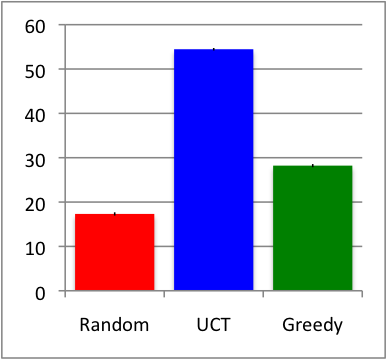
\includegraphics[scale=.55]{figs/random.png}
%\label{fig:UCTvsRANvsGRE}
%}\hspace{5pt}
%\subfigure[]{
%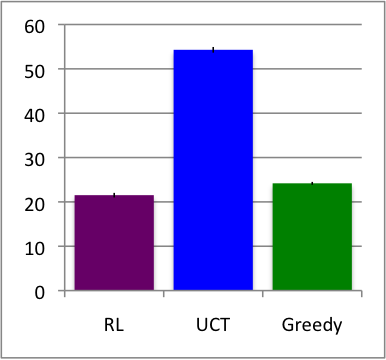
\includegraphics[scale=.55]{figs/rl.png}
%\label{fig:UCTvsRLvsGRE}
%}
%\caption[]{Average Fantasy Risk rewards earned per game ($\times 100$) in contests featuring \subref{fig:UCTvsRANvsGRE}: Random vs.~UCT vs.~Greedy, and \subref{fig:UCTvsRLvsGRE}: RL vs.~UCT vs.~Greedy.}
%\label{fig:FantRisk1}
%\end{figure}  
%
%Figure \ref{fig:FantRisk2} shows the results of two sets of 50 Fantasy Risk rounds of KthBestPick versus Greedy versus UCT$(\cdot, 0.01)$.  In both sets, KthBestPick uses UCT$(3000, 0.25)$ as its heuristic with a fixed arbitrary ordering of the territories to break ties.  The exploration parameter was increased here since it is important for KthBestPick to not only have confidence about the highest ranked pick, but also to have confidence about the next best picks too.  For a fair comparison of KthBestPick and UCT, we instituted a time limit of 250 milliseconds per unowned territory on the board before a pick had to be made.  UCT simply ran as many simulations as possible in the time limit, while KthBestPick iterated on the parameter $N$ of Algorithm \ref{alg:kth}, starting at $N=1$, and returning the last selection made once time was up.  In addition, if a pick of rank $k$ was ever determined to be bad (line 10 or 20), we took the pick of rank $k-1$, simulated this move, and ran UCT simulations from the new state to improve future estimates of actions until time expired.    Furthermore, we ran UCT simulations to rank the picks (line 1) only until at least 3000 simulations had been acquired from the current state, counting previous simulations through this node.  Finally, no program performed any ``thinking'' during another program's turn.
%
%The average rewards shown in Figure \ref{fig:kthOrc} have KthBestPick using itself as the opponent model for all three players, whereas in Figure \ref{fig:KthNoOrc} KthBestPick uses UCT and the logic of Greedy to model its opponents appropriately.  We don't concern ourselves with how KthBestPick would obtain such models here, but only the benefits of having these ``oracles.''  The results of both cases are similar, as KthBestPick beats UCT by a small margin.
%
%\begin{figure}[t]
%\centering
%\subfigure[]{
%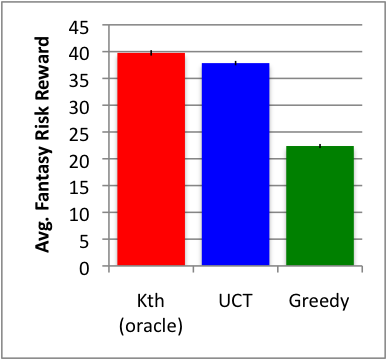
\includegraphics[scale=.55]{figs/kth.png}
%\label{fig:kthNoOrc}
%}\hspace{5pt}
%\subfigure[]{
%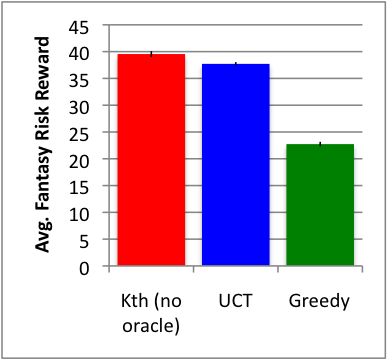
\includegraphics[scale=.55]{figs/kthno.png}
%\label{fig:KthOrc}
%}
%\caption[]{Average Fantasy Risk rewards earned per game ($\times 100$) in contests featuring KthBestPick vs.~UCT vs.~Greedy.}
%\label{fig:FantRisk2}
%\end{figure}
%
%%\subsection{Selfish Play}
%
%% Run experiments, graph results

%\subsection{Full Risk}

% Run experiments of actual Risk results and make graphs

\begin{figure*}[t]
	\centering
	\subfigure[]{
		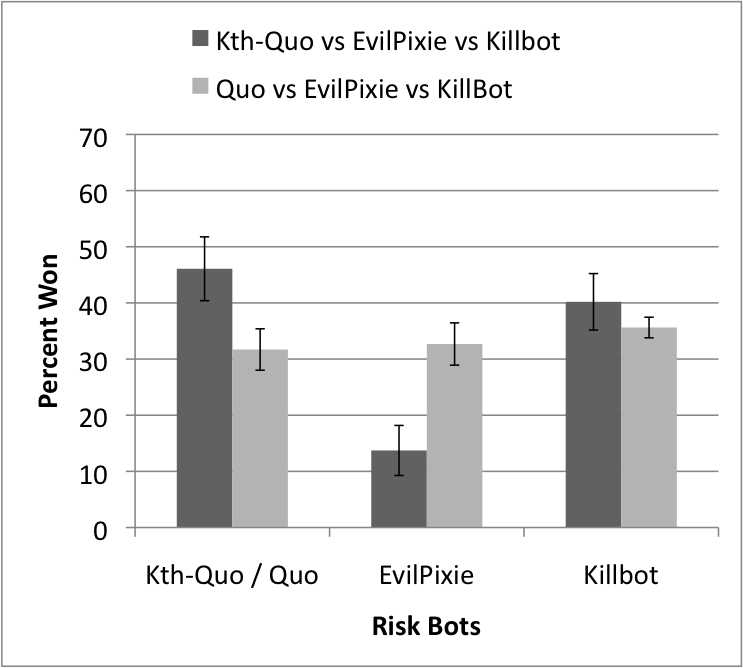
\includegraphics[scale=.4]{figs/KthEvilKillBot.png}
		\label{fig:QuoKthEpKill}
	} %\hspace{5pt}
	\subfigure[]{
		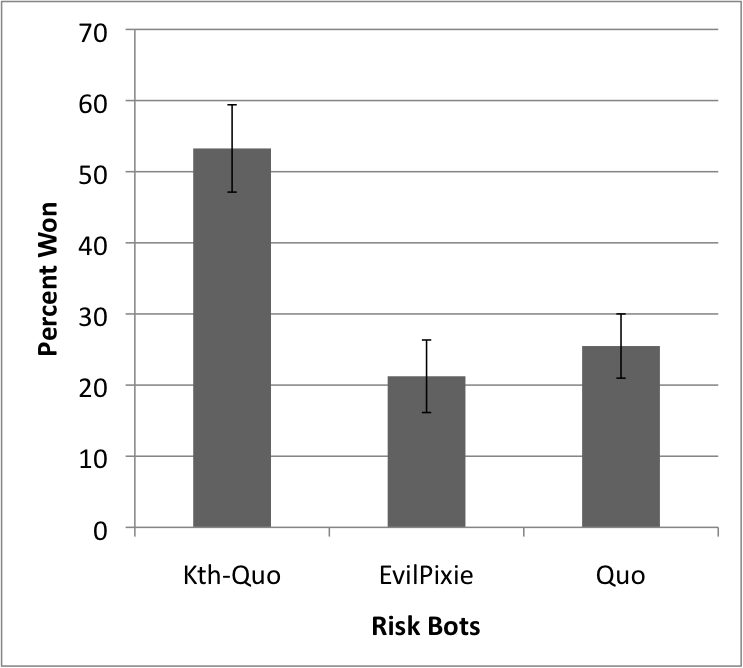
\includegraphics[scale=.4]{figs/KthEvilQuo.png}
		\label{fig:KthQuoEvilP}
	} %\hspace{5pt}
	\subfigure[]{
		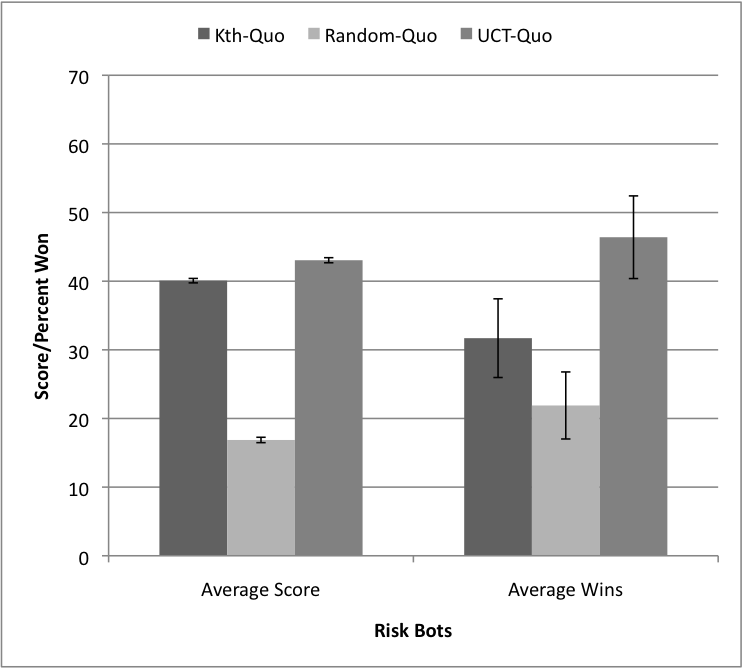
\includegraphics[scale=.4]{figs/KthRandomUCT.png}
		\label{fig:KthUctRan}
	}
	\caption[]{Risk bot performances.  Error bars indicate 95\% confidence intervals.}
	\label{fig:RiskResults}
\end{figure*}

Now that we have a reward signal $r_i(Z)$ to evaluate draft outcomes, we can use UCT to efficiently rank actions within KthBestPick.  As previously described, we created a ``Kth-Quo'' bot by replacing Quo's drafting rules with the KthBestPick algorithm.  For comparison, we also created a ``UCT-Quo'' and a ``Random-Quo'' bot that replace Quo's drafting rules with UCT and a random drafting strategy respectively.  Both UCT-Quo and Kth-Quo used a UCT exploration constant of $c=0.25$, chosen through preliminary experiments.  Kth-Quo also assumes no knowledge of opponents' drafting strategies, resorting to KthBestPick as its opponent models.  In addition to Quo, we pitted Kth-Quo against two other bots labeled as ``difficult'' in the Lux Delux game: Killbot and EvilPixie.  

%We created a ``UCT-Quo'' bot for the full game of Risk by identically duplicating the rule-based strategy of the Quo bot, but replacing its drafting rules with our UCT$(3000,0.01)$ implementation guided by our machine-learned reward signal $r_i(Z)$.  We decided to use UCT rather than KthBestPick so that more games could be played, as KthBestPick requires more time per pick.  

We matched up players in 4 different combinations and for each combination, the winning percentages of each bot over 50 rounds of games are shown in Figure \ref{fig:RiskResults}.  Each round consists of 6 games, one for each of the $3!$ turn orderings of the players.  All games were run with the Lux Delux settings ``selected countries'' and ``placed armies'' turned on, and ``cards'' turned off.  In addition, although Lux Delux does not impose a time limit per turn, we enforce our own time limit of $750 \left \lceil \ell / 3 \right \rceil$ milliseconds, where $\ell$ equals the number of territories left to be picked.  KthBestPick uses exactly 3000 UCT simulations to rank picks and as before, iterates on $N$ until time expires.  All experiments were run on a Pentium Dual-Core CPU 2.1 GHz.  

Figure \ref{fig:QuoKthEpKill} shows that Quo is equally matched against EvilPixie and Killbot, winning roughly one-third of the games against these two opponents.  However, when we pit Kth-Quo against the same two bots, we see in Figure \ref{fig:QuoKthEpKill} that the KthBestPick drafting strategy has, with 95\% confidence, yielded strictly more wins.  In addition, Figure \ref{fig:KthQuoEvilP} shows that despite Quo and Kth-Quo having the same post-draft strategy, Kth-Quo wins roughly 50\% of its matches, about double as many as Quo wins.  Finally, Figure \ref{fig:KthUctRan} shows that unfortunately Kth-Quo loses out to UCT-Quo in terms of both the average reward earned per draft and in number of wins.  We believe this is due to 3000 UCT simulations being an insufficient heuristic for ranking actions in KthBestPick.  With our current time limit, players only have $10.5$ seconds ($\ell = 42$) to make their first pick, which may be too restricting for KthBestPick to use UCT wisely.  Longer time limits and more simulations may narrow the gap that we see in Figure \ref{fig:KthUctRan}; however, more computing resources will be required to test this hypothesis.

%We pitted our UCT-Quo bot against all four bots labeled as ``difficult'' in the Lux Delux game: Killbot, EvilPixie, Quo, and Boscoe.  Each subfigure of Figure \ref{fig:ActualRisk} reports the winning percentage of each bot over 100 rounds (again all 6 turn orderings played each round) Lux Delux with placed initial armies turned on and cards turned off.  Figures \ref{fig:UCTvsQUOvsQUO}, \ref{fig:UCTvsQUOvsEP}, and \ref{fig:UCTvsKILvsBOS} show UCT-Quo winning significantly more than its fair share of games.  In particular, Figure \ref{fig:UCTvsQUOvsQUO} shows that when all players use Quo's post-draft play, a player drafting using UCT guided by $r_i(Z)$ wins frequently against two opponents that follow Quo's rule-based approach (which attempts to draft entire continents when possible).  However, Figure \ref{fig:UCTvsUCTvsQUO} shows that our bot is not perfect, as two UCT-Quo bots lose out to one Quo player.  

%All of our experiments will be conducted in the board game Risk using the Lux Delux\footnote{http://sillysoft.net/lux/} environment.  Lux Delux provides several Risk bots with source code, which include their own hand-coded drafting strategies.  Conveniently, this gives us plenty of competition to test our algorithms against.  We use the selected countries and placed initial armies options in all of our experiments.

%An evaluation function in Risk is provided by (Johansson \& Olsson 2006), and in more detail in (Olsson 2005), to calculate the value of a single territory.  This territory value is meant to approximate how desirable an enemy territory is to a player during gameplay.  The evaluation function is a sum of different sub-components, each measuring a unique situation in the game.  Advantageous situations are given positive values and disadvantageous situations are given negative values.  For example, it is desirable to have more friendly neighbours around a territory, thus the number of friendly neighbours to a territory is a sub-component that contribute positively to the value of this territory.
%We adopted this evaluation function to measure the value of an entire draft to a particular player.  The territory values given by the evaluation function for all territories owned by the player are added together, creating a draft evaluation function.  However, we have to make changes to Johansson \& Olsson's territory evaluation function (from here on referred to as JO) since some sub-components are not longer valid with our new intended purpose:
%\begin{itemize}
%  \item JO gives a value of 0.05 for each army in a friendly neighbour and -0.03 for each army in an enemy neighbour.  Since we are evaluating a complete draft before the post-draft play (where the placing of armies occur), these two components do not apply to us.
%  \item JO gives a value of 20 for owning the whole continent except this territory.  Thus this territory has a high value to the player.  Such a territory is highly desirable since obtaining an entire continent provides a bonus to armies.  In our case, we only give the same value for actually owning the whole continent, since in a final draft all territory ownerships are determined.
%  \item JO gives a value of 4 if an enemy owns the whole continent. In such cases, conquering this enemy territory is desirable since it prevents the enemy from getting the continent army bonus.  In our case, if an enemy owns a continent in the final draft, then it is disadvantageous for the player, so a value of -4 is given.
%\end{itemize}	
%	
%
%\subsection{Analyzing Evaluation Function}
%
%Before we committed to using the new evaluation function as we modified from the paper, we needed to test how well it worked at predicting completed draft states. To test this, we created 6 random draft configurations. These were created by having three agents randomly pick a territory, and then storing the values chosen by each so that they could be recreated later. Therefore, each draft configuration was made up of three sets of draft picks, one for each of the three players (agents). An example map is shown in Figure~\ref{fig:random}. We had a 7th draft configuration where one agent owns an entire continent, in this case Australia, which is shown in Figure~\ref{fig:continent}. 
%
%Next, we computed the evaluation function for each set of picks in each draft. From there, each draft was used to play two sets of 1000 games. The first 1000 games were played such that each agent chose their draft picks based on their turn order, so whichever agent went first on each game chose from set 0. The second set of 1000 games were played such that each agent always choose the same draft picks regardless of order, ie one agent always choose from set 0, one from set 1 and the third from set 2. The number of games each set won for each draft are presented in Table~\ref{tab:results}.
%
%The results show that there are draft combinations that the evaluation function is not taking advantage of, as show in the results for player 2 in set 1, or player 0 in set 2. The other interesting result is that for some draft selections, being the first player (as shown in the ordered results) can be an advantage, something we expected. But, there are cases where a draft set actually does better in the random configuration. By running more tests of the 6 possible orders for the three agents, we may be able to learn more about the advantages/disadvantages the turn order provides. 
%
%%\begin{figure}[htp]
%%\centering
%%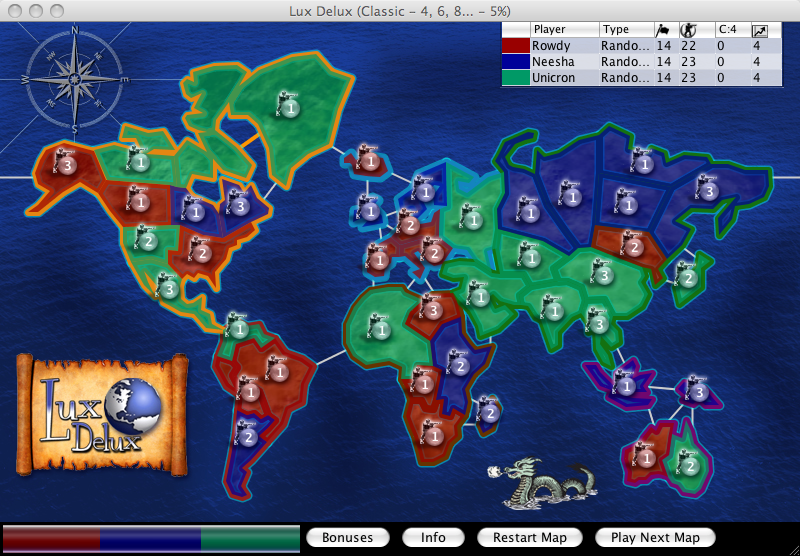
\includegraphics[scale=0.3]{testmap2.png}
%%\caption{Example random draft selection.}\label{fig:random}
%%\end{figure}
%%
%%\begin{figure}[htp]
%%\centering
%%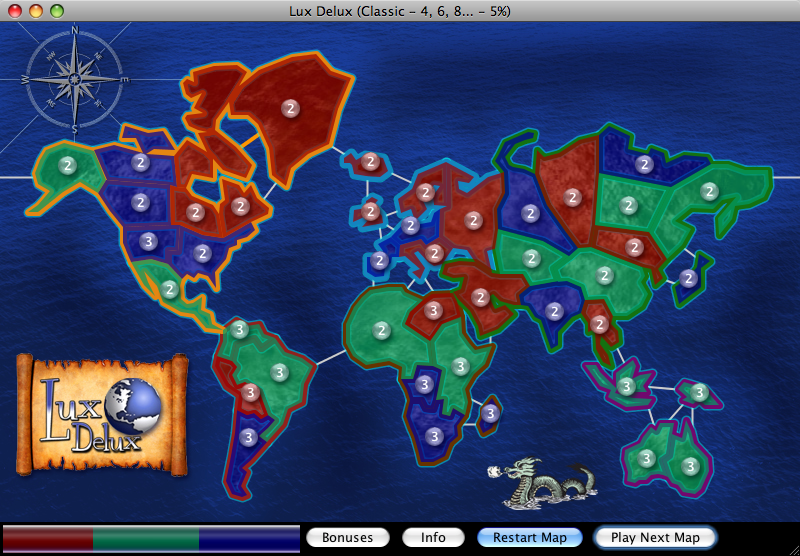
\includegraphics[scale=0.3]{testmapcontinent.png}
%%\caption{Draft selection so that a single player owns a whole continent.}\label{fig:continent}
%%\end{figure}
%
%\begin{table}[]
%%\begin{center}
%%\centering      % used for centering table 
%\begin{tabular}{l l r r r}  % centered columns (5 columns) 
%\hline                       %inserts double horizontal lines
%Draft &  & 0 & 1 & 2 \\[0.5ex]% inserts
%\hline                    % inserts single horizontal line
%0&Evaluation Function&0.278&0.345&0.377\\&Ordered&283&360&357\\&Unordered&420&304&276\\1&Evaluation Function&0.317&0.343&0.34\\&Ordered&322&272&406\\&Unordered&258&309&433\\2&Evaluation Function&0.347&0.342&0.312\\&Ordered&412&354&234\\&Unordered&373&342&285\\3&Evaluation Function&0.323&0.361&0.306\\&Ordered&293&368&339\\&Unordered&347&287&366\\4&Evaluation Function&0.288&0.333&0.379\\&Ordered&330&374&296\\&Unordered&356&368&276\\5&Evaluation Function&0.362&0.302&0.336\\&Ordered&405&356&239\\&Unordered&317&332&351\\6&Evaluation Function&0.195&0.231&0.573\\&Ordered&216&271&513\\&Unordered&247&199&554\\
%[1ex]
%\hline     %inserts single line 
%\end{tabular} 
%%\label{table:nonlin}  % is used to refer this table in the text 
%%\end{center}
%\caption{\label{tab:results} Results of evaluation function and sets on the draft configurations.}
%\end{table}
%
%
%\subsection{Evaluating MaxN-MC using Evaluation Function}
%
%We have run experiments to get an idea of the effectiveness of MaxN-MC using our new evaluation function.  The experiments are set up to have three players.  All three players have identical post-draft strategies provided by a hard-coded Lux agent (namely EvilPixie).  The difference is in the strategies employed in the drafting stage.  While Players 1 and 2 use the hard-coded rules of EvilPixie, Player 0 uses MaxN-MC with our new evaluation function.  Six sets of experiments were run on the world map, each set consisting of 63 to 241 episodes.  An episode is defined as a complete game where each player used their own strategy in the drafting stage then played until a winner is emerged.  
%
%The results are presented in Table~\ref{tab:experiments}.  MAX\_NODES represents the depth in MaxN search where Monte Carlo roll outs take over. NUM\_ROLL\_OUTS represents the number of Monte Carlo roll outs that we average over in MaxN-MC, for each leaf node of the MaxN portion of the search.  A different number of episodes were run for each set of experiments because we have constrained each set to a 24-hour period, and having a larger MAX\_NODES or a larger NUM\_ROLL\_OUTS means that each episode will take longer time.  All experiments show promising results that Player 0 has won a higher number of episodes than the other two players.  Because these results are still preliminary, no conclusions can yet be made.
%
%\begin{table*}[]
%\begin{tabular}{r r r r r r}  % centered columns (6 columns) 
%\hline                       %inserts double horizontal lines
%MAX\_NODES&NUM\_ROLL\_OUTS&Total episodes&Player 0 winning rate&Player 1 winning rate&Player 2 winning rate\\[0.5ex]% inserts
%\hline                    % inserts single horizontal line
%1000&10&190&0.468&0.274&0.258\\
%5000&10&216&0.384&0.361&0.255\\
%10000&10&134&0.425&0.291&0.284\\
%100&100&241&0.432&0.266&0.303\\
%500&100&156&0.423&0.346&0.231\\
%1000&100&63&0.460&0.206&0.333\\
%[1ex]
%\hline     %inserts single line 
%\end{tabular} 
%%\label{table:nonlin}  % is used to refer this table in the text 
%%\end{center}
%\caption{\label{tab:experiments} Results of experiments comparing drafting strategies of MaxN-MC with EvilPixie.}
%\end{table*}

%\section{Discussion}

% Discuss our results, what was interesting, what ideas could carry over to drafting games in general

%Our experiments in Fantasy Risk indicate that UCT and KthBestPick are our best strategies for this game.  While we did run preliminary experiments that indicated an exploration parameter of $c = 0.01$ worked well with 3000 UCT simulations, we did not do the same in the KthBestPick runs.  For these runs, UCT executed well over $3000$ simulations in the time limit and higher exploration here could be beneficial, and so further tests need to be run before we can conclude that KthBestPick is superior.  In addition, it would be interesting to see how often KthBestPick is deviating from the top ranked pick provided by UCT simulations.  Finally, we believe that KthBestPick did not benefit by having ``oracle'' opponent models due to similarities in strategies, particularly between UCT and KthBestPick; however, statistical evidence of this is needed.

% Our RL algorithm failed to achieve satisfactory results in Fantasy Risk. There may be several reasons: the RL method we tried uses a general and naive action and state abstraction mechanism; our evaluation function only produces a reward at the end of a drafting sub-game, once every 14 steps; our RL agent is only trained through self-play. Training against better opponents may speed up convergence.

%In actual games of Risk, our UCT-Quo bot stands ahead of its competition.  When viewing UCT-Quo in action during the draft, it tends to favour territories in North America, while Quo prefers Australia and South America.  In addition, UCT-Quo is often seen preventing an opponent from owning an entire continent by selecting the last territory remaining in the continent.  However, we cannot take all the credit for the high number of victories as we chose Quo for our post-draft play based on its superior winning percentage against the other three difficult bots in preliminary experiments.  Furthermore, two players following our UCT strategy tend to get in each other's way.  For instance, two UCT-Quos will not let each other claim all of North America since they both believe it to be too valuable.  All the while, the other player is able to gather an entire continent or two which may not appear too strong in the eyes of our imperfect reward signal, but ends up proving to be strong picks nonetheless.  We believe this explains the poor performance of the UCT-Quos in Figure \ref{fig:UCTvsUCTvsQUO}.

%\begin{figure}[t]
%\centering
%\subfigure[]{
%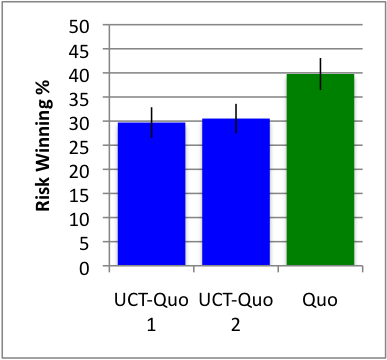
\includegraphics[scale=.55]{figs/2uct.png}
%\label{fig:UCTvsUCTvsQUO}
%}\hspace{5pt}
%\subfigure[]{
%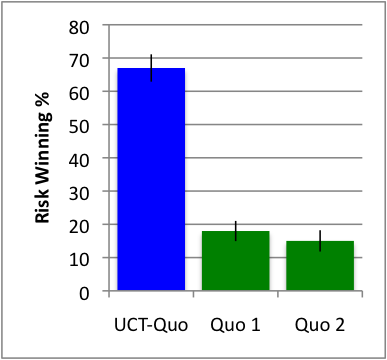
\includegraphics[scale=.55]{figs/2quo.png}
%\label{fig:UCTvsQUOvsQUO}
%}\hspace{5pt}
%\subfigure[]{
%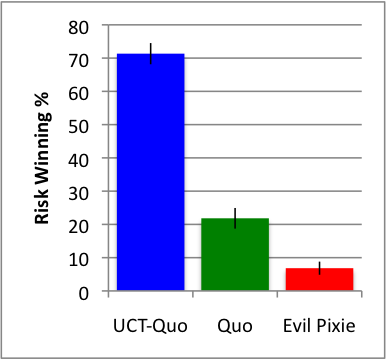
\includegraphics[scale=.55]{figs/evilpixie.png}
%\label{fig:UCTvsQUOvsEP}
%}\hspace{5pt}
%\subfigure[]{
%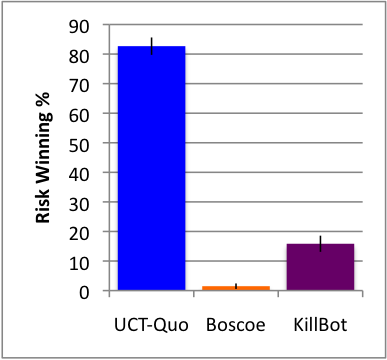
\includegraphics[scale=.55]{figs/others.png}
%\label{fig:UCTvsKILvsBOS}
%}
%\caption[]{Winning percentages in Risk games involving \subref{fig:UCTvsUCTvsQUO}: UCT-Quo vs.~UCT-Quo vs.~Quo, \subref{fig:UCTvsQUOvsQUO}: UCT-Quo vs.~Quo vs.~Quo,  \subref{fig:UCTvsQUOvsEP} UCT-Quo vs.~Quo vs.~Evil Pixie, and \subref{fig:UCTvsKILvsBOS}: UCT-Quo vs.~Boscoe vs.~Killbot.}
%\label{fig:ActualRisk}
%\end{figure}

% Discuss the strengths (and possibly weaknesses) of the approaches.

\section{Conclusions}

% Summarize 

%We formally introduced the concept of a drafting game and showed how to use supervised machine learning to create a reward signal for the drafting sub-game of Risk.  We discussed two strategies, UCT and KthBestPick, for playing drafting games and tested out each in Fantasy Risk, our abbreviated Risk game.  The strongest players in Fantasy Risk were KthBestPick and UCT, and our augmented UCT-Quo bot performed exceptionally well in actual Risk games.

We formally defined the concept of a drafting game and introduced a new algorithm, KthBestPick, specifically for playing drafting games.  KthBestPick performed the best among itself and three other potential strategies in a simple drafting game, particularly in games with lots of initial actions.  Finally, our augmented Kth-Quo Risk bot outperformed several difficult bots provided with Lux Delux, including the Quo bot itself.

%This paper has formalized the concept of a drafting game.    We introduced two solutions for playing a drafting game.  Our first approach, MaxN-MC, is a combination of the MaxN algorithm, which generalizes minimax search to multi-player games, and Monte-Carlo simulations, as used in Monte-Carlo tree search algorithms.  Our second technique is KthBestPick, which uses heuristics to rank actions and opponent models to predict which actions will be selected by other players.  

We see potential future work stemming from using KthBestPick in other drafting-type domains, such as in fantasy sports leagues.  Furthermore, it may be possible try other existing heuristics or develop new means of ranking picks within the algorithm to improve performance in games such as Risk.  Finally, we leave opponent modelling within KthBestPick as another avenue of future research.

%We conclude by listing some possible avenues of further research:
%\begin{itemize} %\addtolength{\itemsep}{-0.5\baselineskip}
%%	\item determine how to model opponents on-line in Fantasy Risk to learn opponent models for KthBestPick.
%	\item apply our techniques to other drafting games, such as drafting in fantasy sports;  %KthBestPick may perform even better in domains where an obvious heuristic exists, such as in the drafting game depicted in Table \ref{tab:KthEx}.  In fantasy sports, actions are usually grouped into types (eg.~a hockey player's position) where each player must select a certain number of actions of each type.  A numerical value (additive reward) is typically associated with each action (eg.~picking a hockey player) estimating the number of points that pick will provide to the fantasy team.  This value provides a simple heuristic for KthBestPick without the need for another algorithm such as UCT.  KthBestPick can then spend all of its efforts determining which of the highest ranked picks to make depending on the number of picks already made of each type by all the players.
%	\item use a more sophisticated classifier for engineering a reward signal, such as an artificial neural network.  This may alleviate the poor performance of UCT-Quo in Figure \ref{fig:UCTvsUCTvsQUO}.%, and would provide a new, likely more complex drafting game to compare algorithms against than our current game of Fantasy Risk.
%%	\item use opponent modelling within UCT.
%\end{itemize}

%\section*{Acknowledgments}
%We would like to thank Vadim Bulitko for directing us to Lee's thesis and for suggesting Fantasy Risk.  %We would also like to thank SillySoft for providing full source code of their Risk bots in Lux Delux.

%\bibliography{../../../LaTeX/bib}
%\bibliographystyle{../../../LaTeX/Styles/aaai}
\bibliography{bib}
\bibliographystyle{aaai}

\end{document}
